\paragraph{} The start of 2021 UCI World Championship time trial is situated on the North Sea beach for both men and woman elite. The women will complete course for a total of 30.30 kilometers with a total elevation gain of 54 meters and men need to finish additional lap for 13 kilometers and elevation gain of 24 meters compared with women's. The whole course is relatively flat which belongs to Cat 4 comparing with Hors Catégorie. Therefore, the energy consumption per kilometer is considered the same under the windless condition on flat ground, which means $E(s)$ always equals $\overline{E}$.
\par By applying our model, we obtain the minimum time to finish race for virtual athletes, shown in table [\ref{time2}].
\begin{table}[h]
	%	\renewcommand\arraystretch{1.3}
	\setlength{\belowcaptionskip}{0.2cm}
	\setlength\tabcolsep{16pt}%调列距
	\centering
	\caption{ Minimum time to finish UCI WCTT}
	\begin{tabular}{ccccc}
		\toprule[2pt]
		&$ T_1$(min)    & $T_2$(min)    & $T_3$ (min)   & Total(min) \\
		\midrule
		MTT   & 27:23 & 15:07 & 7:05  & 49:35 \\
		FTT   & 26:21 & 3:17  & 8:49  & 38:27 \\
		\bottomrule[2pt]
	\end{tabular}%
	\label{time2}%
\end{table}%

\par As is shown in table [\ref{time2}], our virtual male cyclist applies power at the level of FTP in the first 27:23(min), the recovers for 14:07(min)and finally makes all-out effort to the end. His total result is 48:36(min). Results of female cyclist can be interpreted similarly.
\begin{figure}[h]
	\centering
	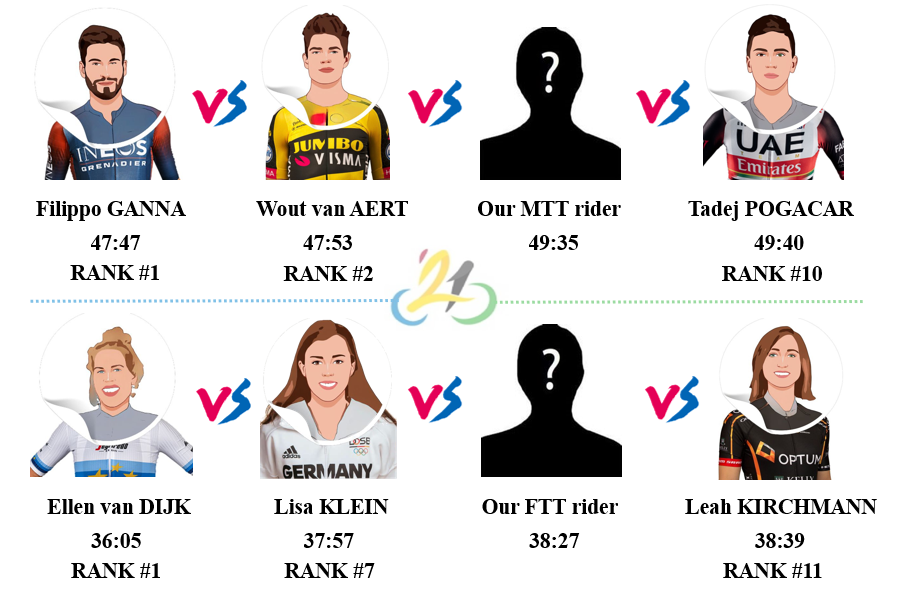
\includegraphics[width=0.9\linewidth]{image/rider1}
	\caption{Our virtual riders and participants of 2021 UCI World Championship time trial}
	\label{rider1}
\end{figure}
\par In order to verify the rationality and reliability of our model, we compare the score with ITT racers in 2021 UCI World Championship time trial as the graph presented [\ref{rider1}]---our MTT and FTT rider rank 5 and 10 respectivly.
% TODO: \usepackage{graphicx} required
